\subsection{First Research Question}
\label{sec:ResearchQuestion1}
The first research question of this project states:
\\
"How well can dynamic networks be modelled using a Stepwise Constant Velocity Model (SCVM) representation in Euclidean latent space?"
\\\\
In order to answer this question, the modelling approach will be evaluated on synthetically generated data.
Here synthetic dataset 1 is utilized, which is synthesized using a single velocity vector, as explained in section \ref{sec:Data:SyntheticData:SyntheticDataset1}.

\subsubsection{Modelling of single-step synthetic data}
\label{sec:ResearchQuestion1:singleStepSynthetic}
The first part of answering research question one consists of confirming proper modelling performance of a single step stepwise Constant Velocity Model.
This is done as an initial procedure as it lays the foundation of the SCVM, meaning if the single-step model does not work as intended, the multi step modelling will neither.
\clearpage
\noindent
\textbf{Loss and beta convergence results}
\\
The single step SCVM has been trained for 5000 epochs on the full dataset 1 as one training batch using a single velocity step and a learning rate of 0.025. The model is compared against a baseline model which is simply a model with no dynamics i.e. a model with no velocity. Also for comparison the ground truth with the correct starting positions and velocity from the data synthesization is provided.
Below, table \ref{tab:SingleStep1}, shows the learned beta parameter and final negative log loss, including that of the ground truth model.

\begin{table}[H]
\centering
\begin{tabular}{|l|c|cc|}
\hline
Model         & \multicolumn{1}{l|}{Num. Epochs} & Beta & Avg. NLL \\ \hline
Ground Truth  & -                                & 7.5  & -82377.99  \\
No V Baseline & 5000                             & 6.487  & 34715        \\
1 Step Model  & 5000                             & 7.495   & -82376.19      \\ \hline
\end{tabular}
\caption{Final learned $\beta$ value and negative log loss for baseline trained model.}
\label{tab:SingleStep1}
\end{table}
Here the single step SCVM more or less converge to the precise beta value and prove much better than the no velocity baseline, which is no way near the correct beta.
\\\\
\noindent
\textbf{Intensity rate comparison results}
\\
The intensity rates for 5000 epochs training of the baseline model:
\begin{figure}[H]
    \centering
    \begin{subfigure}[b]{\textwidth}
        \centering
        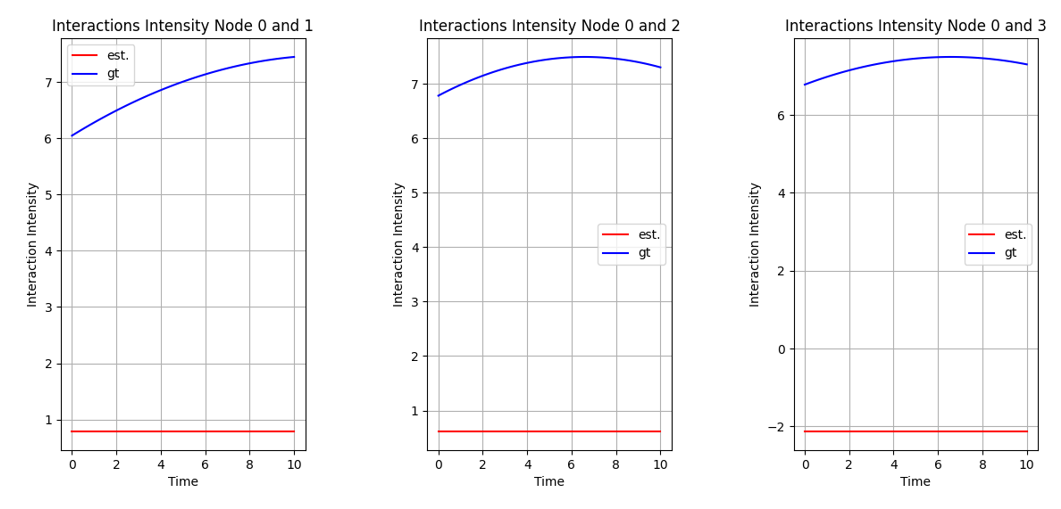
\includegraphics[width=\textwidth]{0_images/rq1_baseline_intensity_plot1.png}
    \end{subfigure}
    \vfill
    \begin{subfigure}[b]{\textwidth}
        \centering
        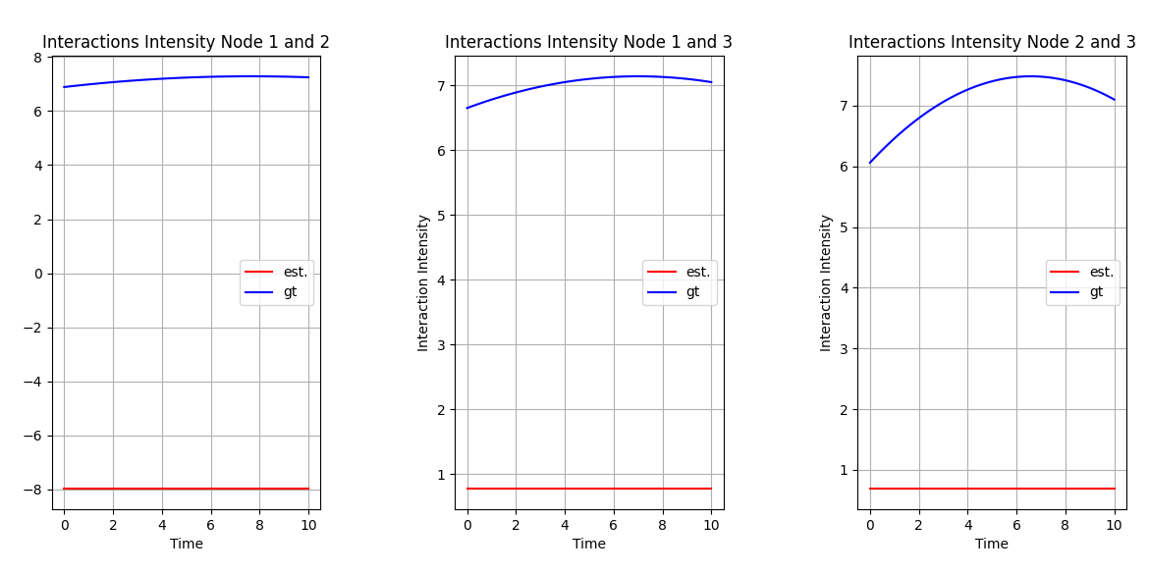
\includegraphics[width=\textwidth]{0_images/rq1_baseline_intensity_plot2.png}
    \end{subfigure}
    \caption{Basline model's node pair interaction intensity for synthetic dataset 1 trained for 5000 epochs. Blue line is the ground truth model, red is the baseline model.}
    \label{fig:RQ1:baseline_intensity}
\end{figure}
\noindent
Intensity rates for 5000 epochs single step SCVM model training:
\begin{figure}[H]
    \centering
    \begin{subfigure}[b]{\textwidth}
        \centering
        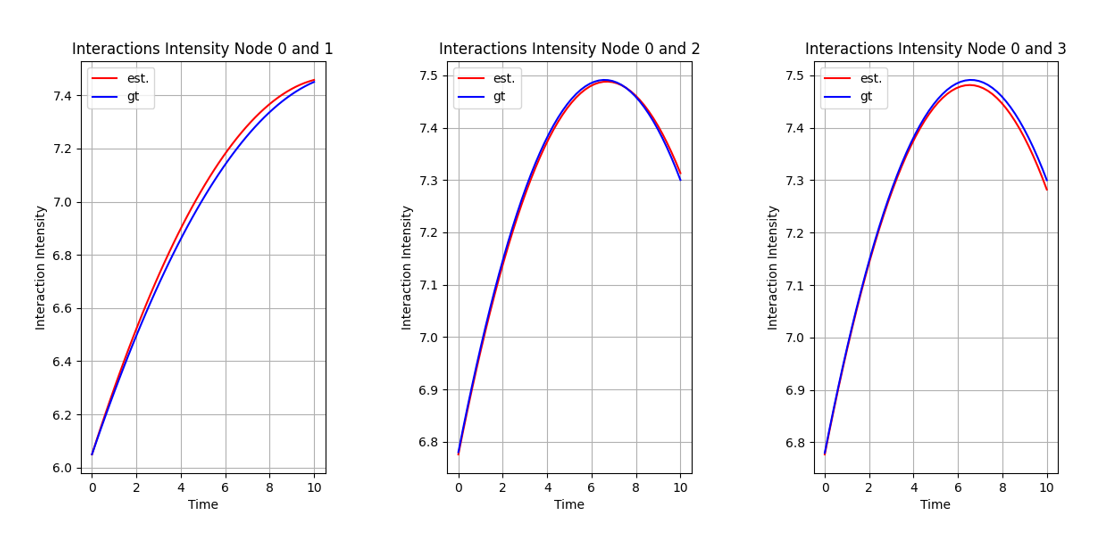
\includegraphics[width=\textwidth]{0_images/rq1_SCVM_intensity_plot1.png}
    \end{subfigure}
    \vfill
    \begin{subfigure}[b]{\textwidth}
        \centering
        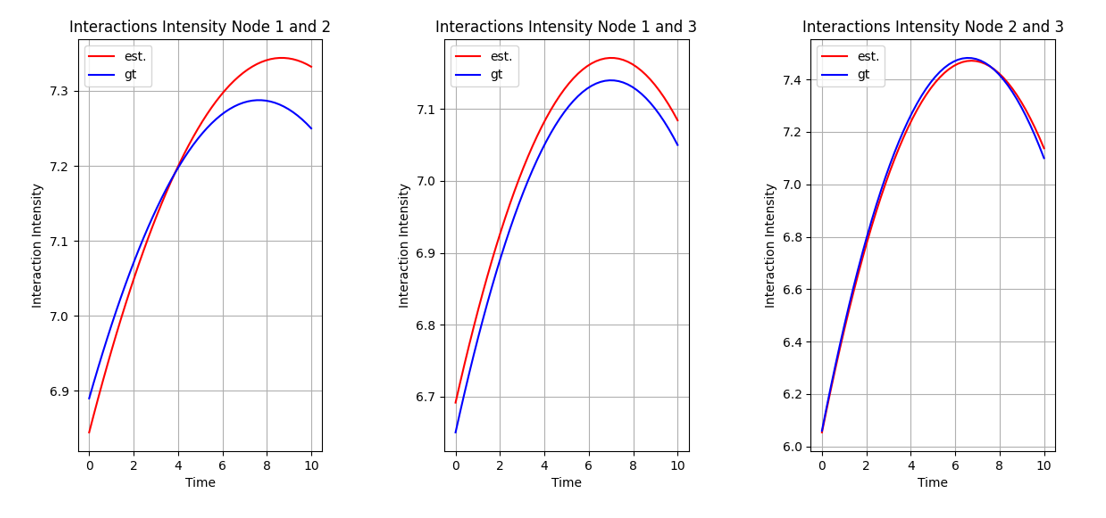
\includegraphics[width=\textwidth]{0_images/rq1_SCVM_intensity_plot2.png}
    \end{subfigure}
    \caption{SCVM model's node pair interaction intensity for synthetic dataset 1 trained for 5000 epochs. Blue line is the ground truth model, red is the model estimation.}
    \label{fig:RQ1:SCVM_intensity}
\end{figure}
\noindent
The interaction intensity plots supports the performance of the single SCVM being much better then the no velocity model.
\\\\
\textbf{Interaction removal results.}
\\
The results from interaction removal, as explained in \ref{sec:Method:Evaluation:AUC}, shows a worse than random accuracy for the no velocity baseline model:
\begin{figure}[H]
    \centering
    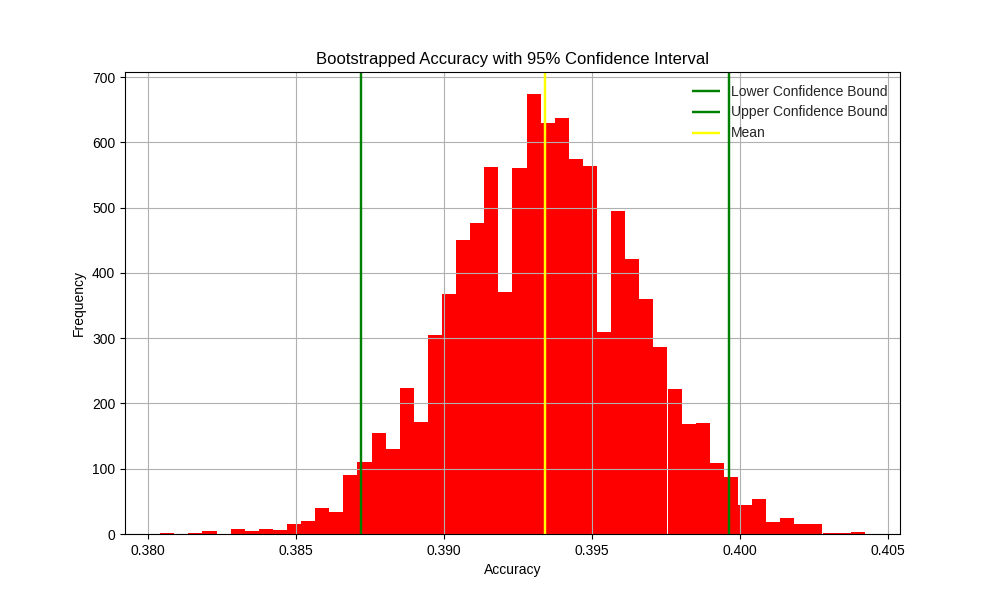
\includegraphics[width=0.8\textwidth]{0_images/rq1_baseline_accuracy.png}
    \caption{Baseline model's interaction removal accuracy 95 \% confidence for synthetic dataset 1 trained for 5000 epochs.}
    \label{fig:RQ1:baseline_accuracy}
\end{figure}
\noindent 
The single step SCVM has a better, but still low accuracy, for predicting the correct node pair interaction.
\begin{figure}[H]
    \centering
    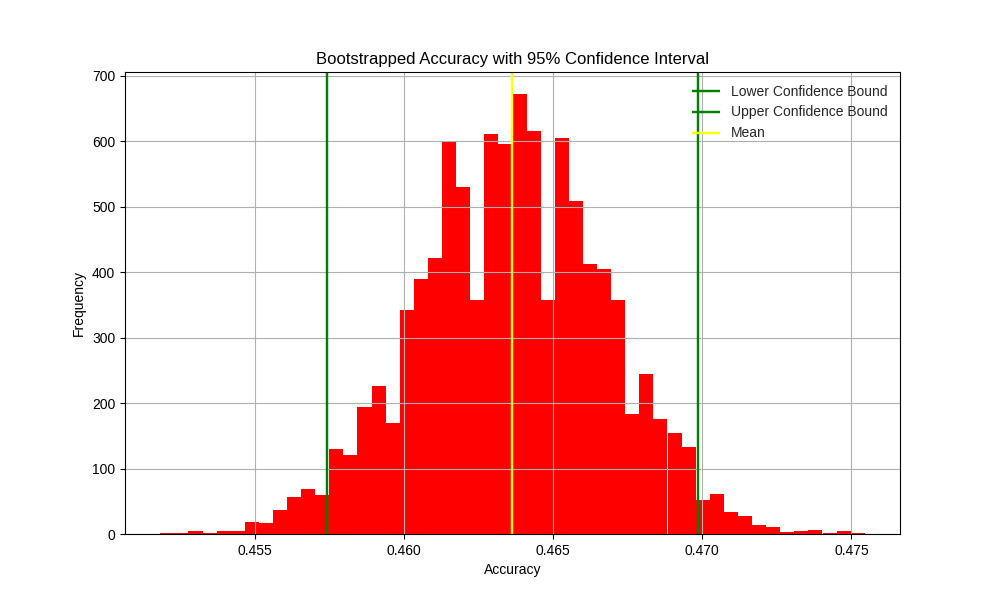
\includegraphics[width=0.8\textwidth]{0_images/rq1_SCVM_accuracy.png}
    \caption{Single step SCVM model's interaction removal accuracy 95 \% confidence for synthetic dataset 1 trained for 5000 epochs.}
    \label{fig:RQ1:SCVM_accuracy}
\end{figure}
\noindent
However a difference for the SCVM compared to the basline is, that the single step SCVM actually achieves an accuracy similar to that of the ground truth model.
\begin{figure}[H]
    \centering
    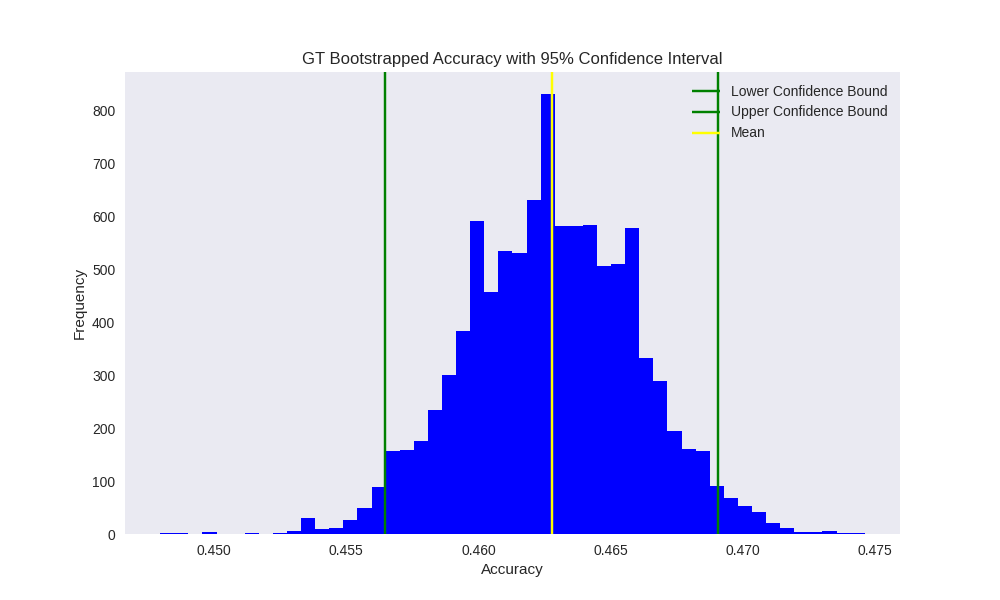
\includegraphics[width=0.8\textwidth]{0_images/rq1_GT_accuracy_SCVM.png}
    \caption{Ground truth model interaction removal accuracy 95 \% confidence interval for synthetic dataset 1}
\end{figure}
\noindent
As both models are within a 46-47 \% accuracy confidence interval in the tests.
\\\\
\noindent
\textbf{Dyad removal results}
\\
\noindent
The baseline that has no dynamics is killed here, as it is not even able to be interpreted properly in the dyad removal test, where node pairs are removed across time. Instead we only look at the resulting node interaction intensity plots for the single step SCVM:
\begin{figure}[H]
    \centering
    \begin{subfigure}[b]{\textwidth}
        \centering
        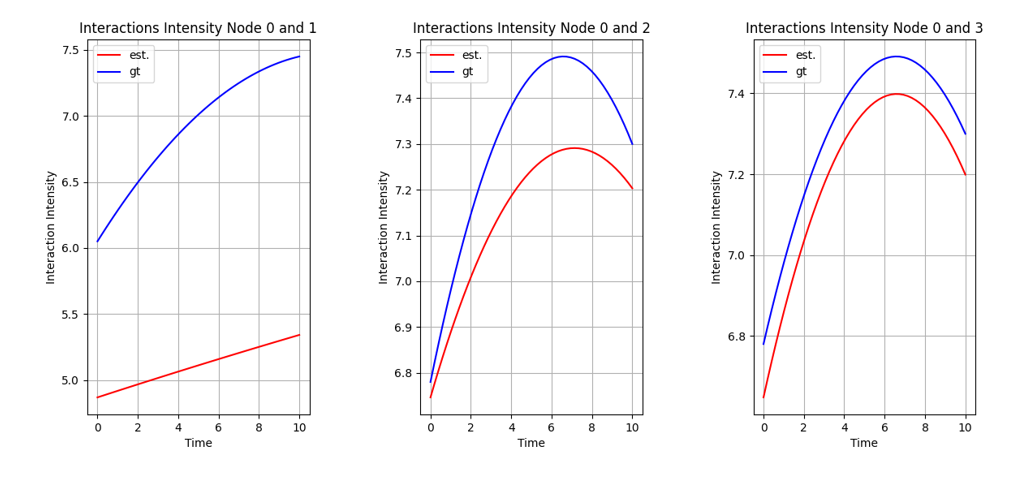
\includegraphics[width=\textwidth]{rq1_dyad_removal_SCVM1.png}
    \end{subfigure}
    \hfill
    \begin{subfigure}[b]{\textwidth}
        \centering
        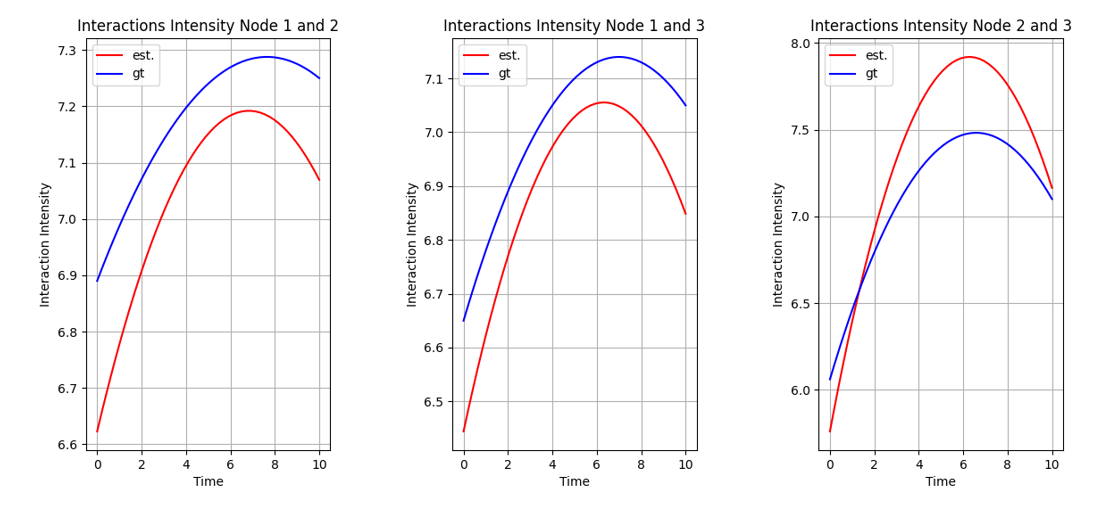
\includegraphics[width=\textwidth]{rq1_dyad_removal_SCVM2.png}
    \end{subfigure}
        \caption{SCVM intensity plot after removing node pair (0,1)}
    \label{fig:RQ1:SCVM_accuracy}
\end{figure}
\noindent
The plot shows a clear negative impact on the fitting of the interaction intensity for the removed node pair, i.e. the model is not quite cabable of interpreting their interaction intensities from the remaining node pair interactions.

\subsubsection{Multi-step TDGN modelling of synthetic data}
\label{sec:ResearchQuestion1:multiStepSynthetic}
The second part of answering the first research question evaluates the SCVM with 10 steps to test its capabilities with multiple steps. The model is matched against the single step SCVM from earlier, and a ground truth 10 step SCVM is also provided. 
The test uses the synthetic dataset 2, see section \ref{sec:Data:SyntheticData:SyntheticDataset2}.
\\\\
\textbf{Loss and beta convergence results}

\begin{table}[H]
\centering
\begin{tabular}{|l|c|cc|}
\hline
Model         & \multicolumn{1}{l|}{Num. Epochs} & Beta & Avg. NLL \\ \hline
Ground Truth  & -                                & 7.5  & -192208.05 \\
Single Step SCVM & 5000                          & 6.971 &  -153453.037      \\
10 Step SCVM & 5000                          & 7.499   & -191501.75      \\ \hline
\end{tabular}
\caption{Learned $\beta$ value and negative log loss for models on synthetic dataset 2 \ref{sec:Data:SyntheticData:SyntheticDataset2}}
\label{tab:MultiStep1}
\end{table}
\noindent 
The convergence results now clearly shows the limitation of the single step SCVM, as the synthetic data has changed to be generated with several velocities, the model no longer converge to the correct beta value, and receives a worse NLL. On the other hand, the 10 step SCVM shows a fint NLL and convergence to the correct beta.
\\\\
\textbf{Intensity rate comparison results}
\\\\
Investigating the interaction intensity plots for the two models also, supports the convergence findings.
\\\\
The intensity rates for 5000 epochs training of the single step SCVM:
\begin{figure}[H]
    \centering
    \begin{subfigure}[b]{\textwidth}
        \centering
        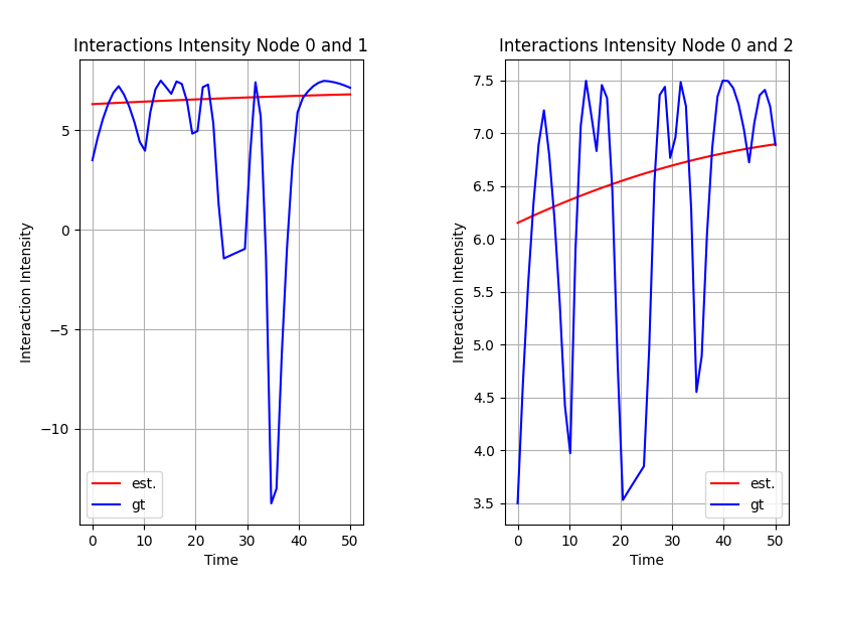
\includegraphics[width=\textwidth]{0_images/rq1_2_1step_intensity_plot_node_01_02.PNG}
    \end{subfigure}
    \vfill
    \begin{subfigure}[b]{\textwidth}
        \centering
        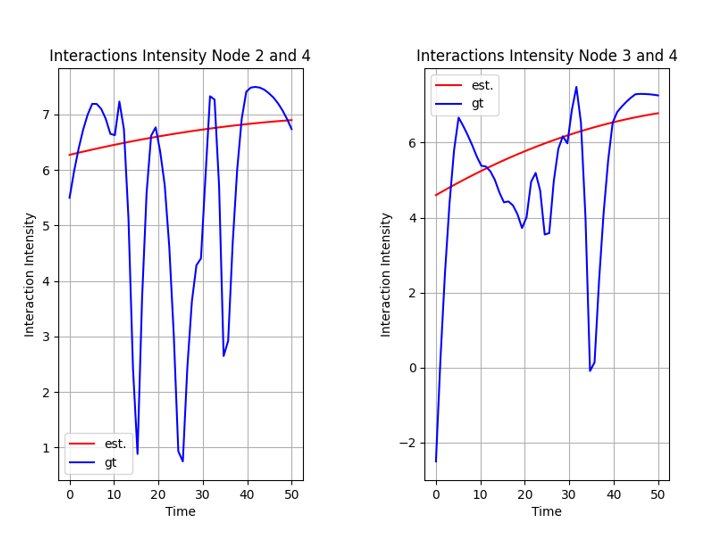
\includegraphics[width=\textwidth]{0_images/rq1_2_1step_intensity_plot_node_23_34.PNG}
    \end{subfigure}
    \caption{Single step SCVM model's node pair interaction intensity for synthetic dataset 2 trained for 5000 epochs. Blue line is the ground truth model, red is the model estimation.}
    \label{fig:RQ1:part2:1step_intensity}
\end{figure}
\noindent
The single step SCVM is clearly limited by only having a single velocity to fit.
For all interaction intensity plots from the single step SCVM  see appendix \ref{appendix:rq1:part2:1step_intensity}.
\\\\
The intensity rates for 5000 epochs training of the 10 step SCVM:
\begin{figure}[H]
    \centering
    \begin{subfigure}[b]{\textwidth}
        \centering
        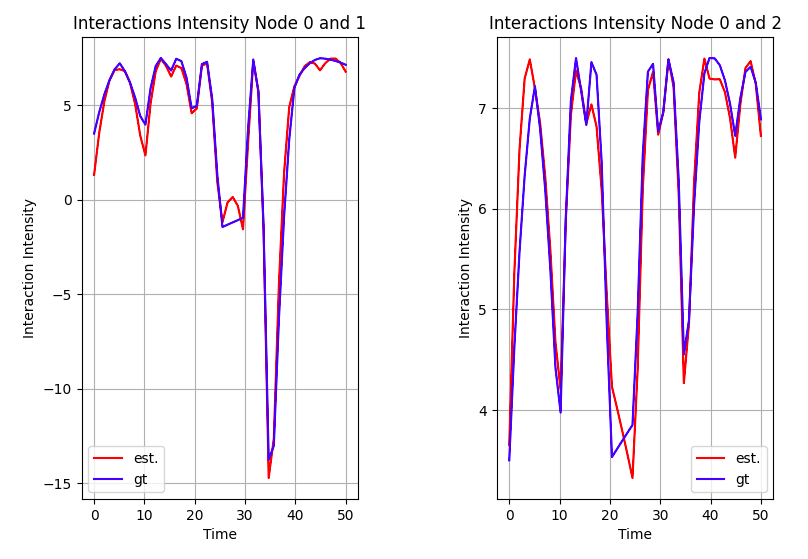
\includegraphics[width=\textwidth]{0_images/rq1_10step_SCVM_intensity1.png}
    \end{subfigure}
    \vfill
    \begin{subfigure}[b]{0.45\textwidth}
        \centering
        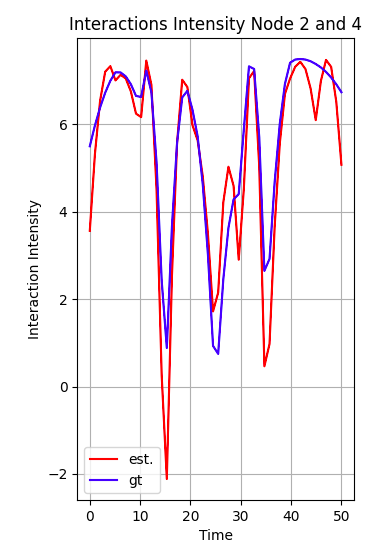
\includegraphics[width=\textwidth]{0_images/rq1_10step_SCVM_intensity3.png}
    \end{subfigure}
    \hfill
    \begin{subfigure}[b]{0.45\textwidth}
        \centering
        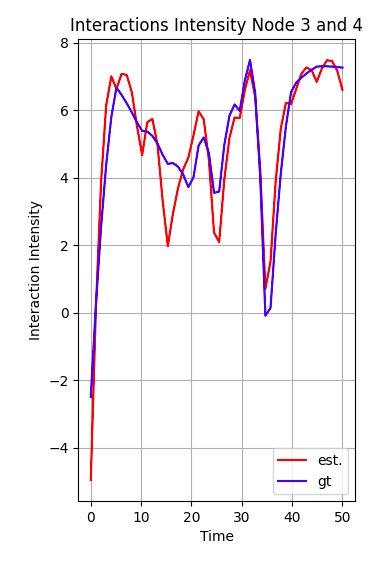
\includegraphics[width=\textwidth]{0_images/rq1_10step_SCVM_intensity2.png}
    \end{subfigure}
    \caption{10 step SCVM model's node pair interaction intensity for synthetic dataset 2 trained for 5000 epochs. Blue line is the ground truth model, red is the model estimation.}
    \label{fig:RQ1:part2:10step_intensity}
\end{figure}
\noindent
Here the model clearly benefits from having multiple velocities to fit the node pair intensities. To see all interaction intensity plots for the 10 step SCVM see appendix \ref{appendix:rq1:part2:10step_intensity}
\\\\
\noindent
\textbf{Interaction removal results}
\\
The accuracy on removed interactions for the single step SCVM model:
\begin{figure}[H]
    \centering
    \centering
    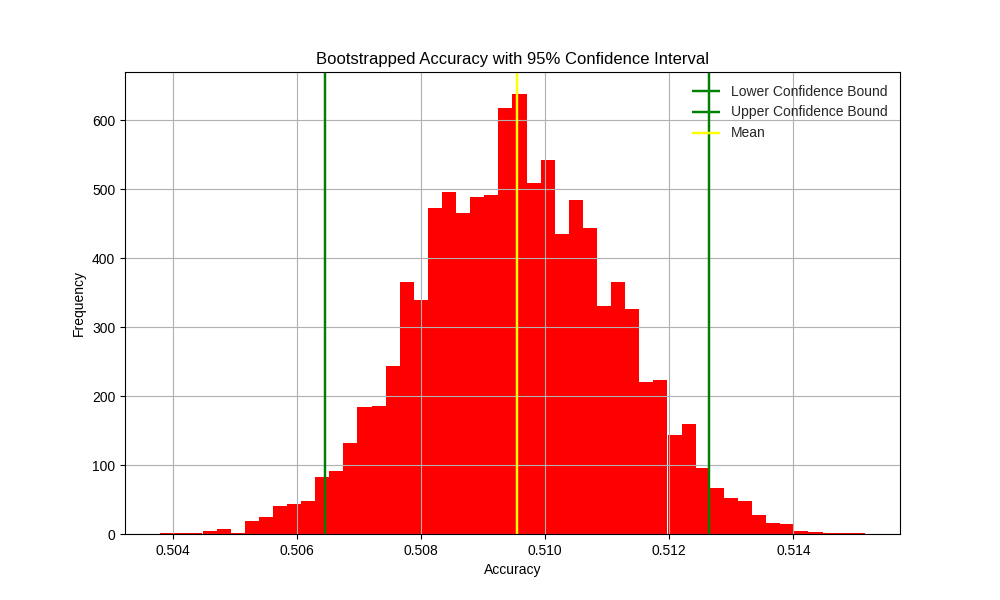
\includegraphics[width=0.8\textwidth]{0_images/rq1_2_1step_accuracy_plot.png}
    \caption{Single step SCVM model's interaction removal accuracy 95 \% confidence for synthetic dataset 2 trained for 5000 epochs.}
    \label{fig:RQ1:1step_SCVM_accuracy}
\end{figure}
\noindent
The accuracy confidence interval shows an accuracy of the single step model which is around random. 
\clearpage
The accuracy on removed interactions for the 10 step SCVM model:
\begin{figure}[H]
    \centering
    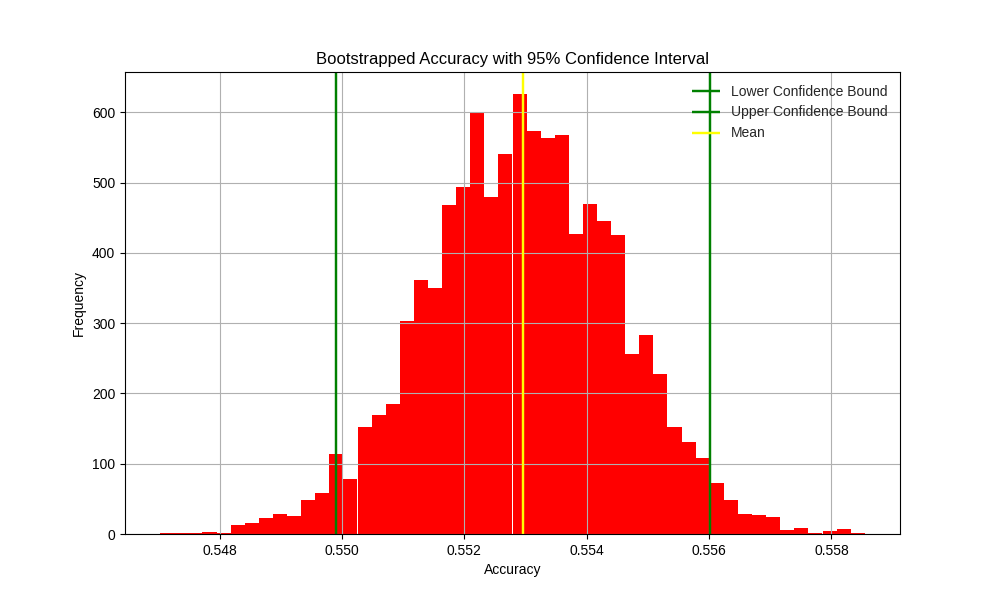
\includegraphics[width=0.8\textwidth]{0_images/10step_SCVM_Accuracy_Plot.png}
    \caption{10 step SCVM model's interaction removal accuracy 95 \% confidence interval for synthetic dataset 2 trained for 5000 epochs.}
    \label{fig:RQ1:SCVM_accuracy}
\end{figure}
\begin{figure}[H]
    \centering
    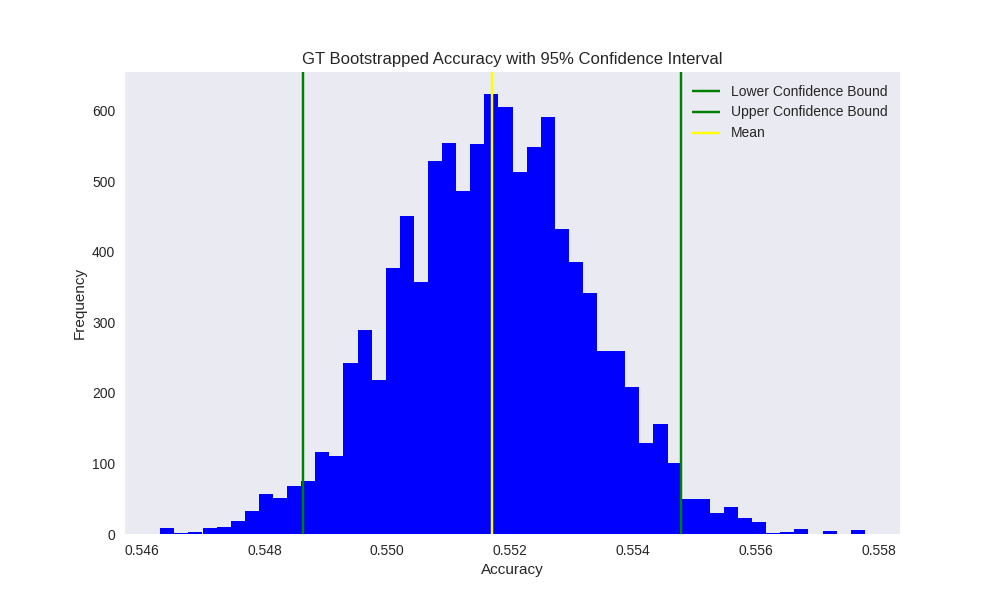
\includegraphics[width=0.8\textwidth]{0_images/10step_SCVM_GT_Accuracy_Plot.png}
    \caption{Ground truth interaction removal accuracy 95 \% confidence interval for synthetic dataset 2}
\end{figure}
\noindent
Here we also see an accuracy close to random for the 10 step model. However, the accuracy of the model matches that of the ground truth, which also only achieves around 55 \% accuracy on the synthetic dataset 2.
\clearpage
\noindent
\textbf{Dyad removal results}
\\
The interaction intensity fits after dyad removal for the single step SCVM were just as bad as for the initial fits, where no dyads were removed. Which again speaks to the limitation of the single step SCVM when fitting data with multiple veclocity changes. 
To see the interaction intensity plots for the single step SCVM after removal of node dyad (0,2) see appendix \ref{appendix:rq1:part2:1step_dyad_remove}.
\clearpage
\noindent
The dyad removal results for 10 step SCVM:
\begin{figure}[H]
    \centering
    \begin{subfigure}[b]{\textwidth}
        \centering
        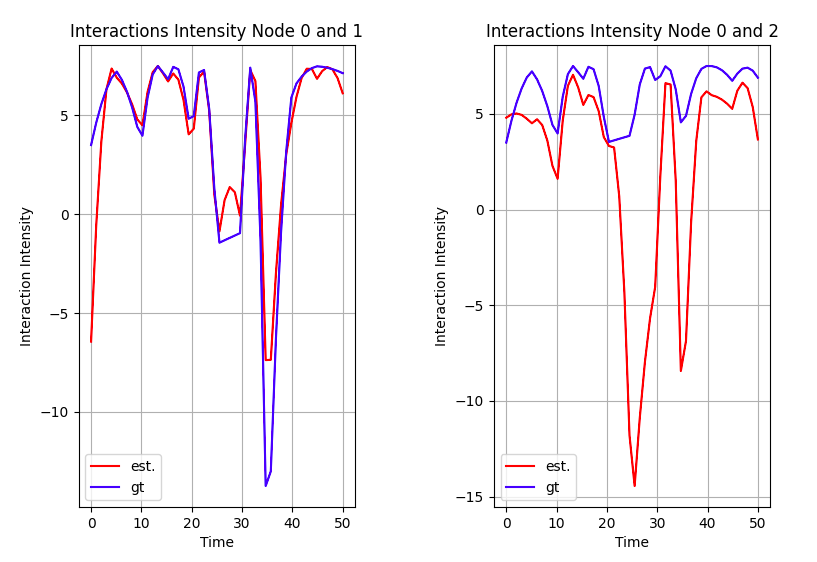
\includegraphics[width=0.8\textwidth]{0_images/10step_SCVM_dyad_removal_plot1.png}
    \end{subfigure}
    \hfill
    \begin{subfigure}[b]{\textwidth}
        \centering
        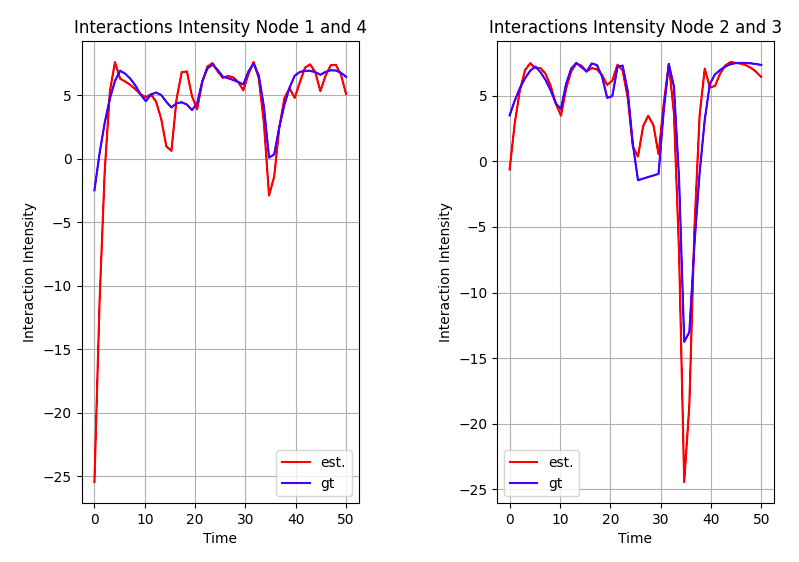
\includegraphics[width=0.8\textwidth]{0_images/10step_SCVM_dyad_removal_plot2.png}
    \end{subfigure}
        \caption{10 step SCVM intensity plot after removing node pair (0,2)}
    \label{fig:RQ1:SCVM_accuracy}
\end{figure}
\noindent
Here the 10 step SCVM does not have too much truble fitting the kept node pairs, but it still struggles with parts of the intensity for the removed dyad (0,2). For all interaction intensity plots of the dyad removal see appendix \ref{appendix:rq1:part2:10step_dyad_remove}.


\subsubsection{Multi-step modelling of real world data}
\label{sec:ResearchQuestion1:ResistanceTraining}
The third part of answering the first research question investigates the SCVM's modelling capabilities on a real world dataset using 100 velocity steps. 
The dataset used for testing is the real dataset 1, the resistance game, presented in section \ref{sec:Data:RealData:RealDataset1}.
\\\\
\textbf{Interaction removal results}
\\
Since the dataset is a real life dataset, there is now ground truth as with the synthetic data. Therefore the 100 step SCVM is evaluated using the interaction removal test:
\begin{figure}[H]
    \centering
    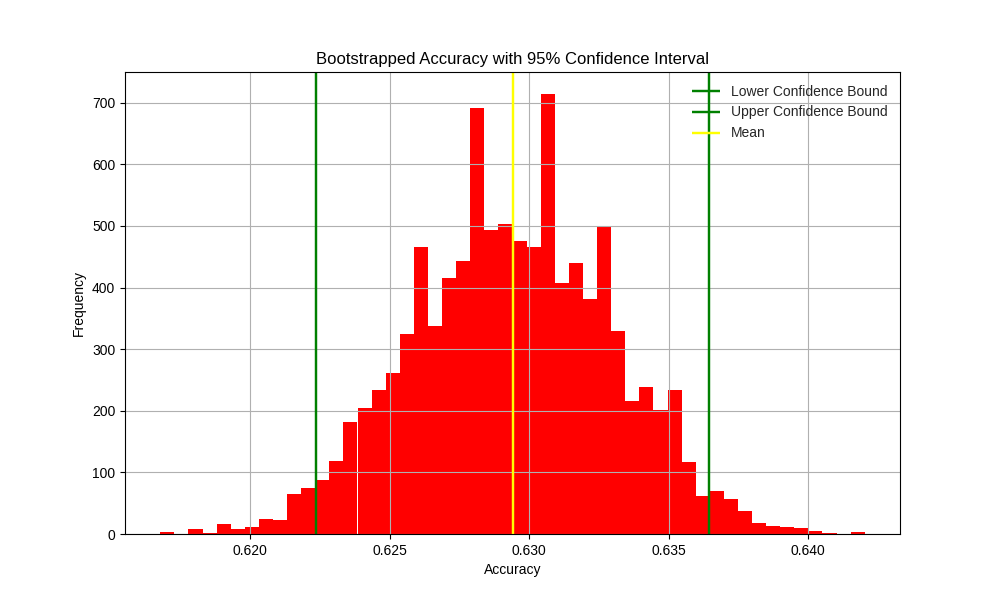
\includegraphics[width=\textwidth]{0_images/100steps_SCVM_real_dataset_accuracy_plot.png}
    \caption{100 step SCVM model's interaction removal accuracy 95 \% confidence for real dataset 1 trained for 5000 epochs.}
    \label{fig:RQ1:SCVM_accuracy}
\end{figure}
\noindent
For the real dataset 1, the SCVM model achieves an accuracy score of around 63 \%, which is an improvement compared to a random baseline of 50 \% and compared to the performance on the synthetic datasets.